\chapter{POISE}
\label{chpt:poise}

This chapter describes the development of software for on-the-fly optimisation of NMR experimental parameters, titled POISE (\textit{Parameter Optimisation by Iterative Spectral Evaluation}).
The primary benefit of this is that parameters may be adjusted for individual spectrometers and samples, which may vary greatly in their chemical properties.
POISE is primarily written in Python 3.
In this chapter, I first provide some details about the implementation of POISE.
The bulk of the text which follows is devoted to a number of applications in liquid-state NMR spectroscopy.
At the end, the extension of the concept of on-the-fly optimisation to ESR spectroscopy is also briefly discussed: I contributed code for this, but the experimental ESR work and data analysis were carried out by Jean-Baptiste Verstraete (University of Oxford).

The work in this chapter forms the subject of two publications:

\begin{itemize}
    \item \fullcite{Yong2021AC}
    \item (JBV et al., manuscript submitted)
\end{itemize}

\clearpage

\section{Introduction}
\label{sec:poise__introduction}

In the previous chapter, I covered various approaches to improving pure shift NMR through the use of optimisation.
Although the optimisation code written there was highly specialised and only designed to work on pure shift applications, it was envisioned that this optimisation approach could be applied to essentially \textit{any} NMR experiment where parameter optimisation was required.
In principle, this description is appropriate for \textit{every} experiment: even the simplest pulse--acquire experiment can be optimised through the use of Ernst angle excitation.
More complex examples, such as 2D experiments, typically have parameters which should be chosen to optimally match coupling constants (INEPT delay) or relaxation rates (NOE mixing time).

In practice, the need for accurate parameters is often `solved' through the use of compromise values, which typically fall in the middle of an expected range for typical molecules.
For example, these values may be stored as part of a parameter set designed to be reused.
Alternatively, parameter values may be optimised `by hand'.
However, compared to these, the use of experimental optimisation has several benefits.
It is:
\begin{enumerate}
    \item \textit{sample-specific}, and as long as the default values are within the optimisation bounds, the optimisation will yield performance which is no worse than the defaults;
    \item more \textit{robust} towards unusual molecular structures, which have physical or chemical properties which fall outside of an expected range;
    \item \textit{instrument-specific}, so can compensate for spectrometer imperfections.
    \item \textit{automated}, so does not require an expert to adjust parameter values manually, or even any user intervention for that matter;
    \item \textit{objective}, in that the quality of a spectrum can (in principle) be mathematically measured through a cost function; and
    \item \textit{fast}, in that it uses an algorithm which is designed to achieve rapid decreases in the objective function: many `manual' optimisations involve either trial-and-error or an exhaustive grid search (i.e.\ increasing a parameter value one step at a time), neither of which are efficient.
\end{enumerate}

Despite these advantages, experimental optimisation of NMR parameters has seen only limited use.
In fact, although there are several examples of such optimisations in laser\autocite{Bardeen1997CPL}, nuclear quadrupole resonance\autocite{Schiano1999JMR,Schiano2000ZNA,Monea2020JMR}, and ESR\autocite{Goodwin2018JMR} spectroscopies, 
the only direct parallel in NMR which I have found is that of the eDUMBO pulses for heteronuclear\autocite{DePaepe2003CPL,Elena2004CPL} and homonuclear dipolar\autocite{Salager2010CPL} decoupling in solid-state MAS experiments.
In this work, the Emsley group used `direct spectral optimisation' (equivalent to what I call `experimental optimisation') to determine the best coefficients for a Fourier series pulse.
The performance of these pulses was measured by a cost function which (primarily) took into account the intensity of the detected peaks: a larger intensity corresponds to better decoupling performance.
Interestingly, the aim of using an experimental optimisation here was not to obtain sample-specific pulses (point (1)), but rather to account for the `spectrometer response', i.e.\ instrumental non-idealities (point (3)).
It was assumed that the compound used for the optimisation was a suitably representative choice, so that the optimisation result could simply be applied to other samples with no change.

The likely reason for the low popularity of experimental optimisations is \textit{time}.
Each \textit{function evaluation} (FE), i.e.\ each measurement of the cost function, corresponds to the acquisition of an NMR spectrum which may take seconds to minutes.
In most cases, it is probably easier to run NMR optimisations in a theoretical manner, which can be much faster and also circumvents the effect of noise.
Examples of such optimisations include the design of shaped pulses through optimal control theory\autocite{Skinner2003JMR,Khaneja2005JMR,Kobzar2008JMR,Kobzar2012JMR,Schilling2014ACIE,Glaser2015EPJD}, by simple parameterisation\autocite{Geen1989JMR,Emsley1990CPL,Geen1991JMR,Nuzillard1994JMRSA,Kupce1995JMRSA,Kupce1995JMRSB}, or the optimisation of entire pulse sequences\autocite{Shaka1985JMR,Freeman1987JMR,Bechmann2013JMR,Ehni2014JMR,Lapin2020JMR} (this is essentially what I did with the dPSYCHE experiment in \cref{sec:pureshift__dpsyche}).
(In fact, even the aforementioned eDUMBO pulses were not \textit{originally} designed as an experimental optimisation: they are actually an enhancement of the DUMBO decoupling schemes, which were optimised using numerical simulations\autocite{Sakellariou2000CPL}.)

In this chapter, I aim to provide a convincing argument that experimental optimisation is not necessarily slow.
In particular, I will show that it is often possible to devise optimisation routines which yield improved results in a matter of minutes.
All the optimisations here are performed using a software package written by me, called POISE (Parameter Optimisation by Iterative Spectral Evaluation).
POISE is open-source (\url{https://github.com/foroozandehgroup/nmrpoise}) and can be installed in a single step through \texttt{pip install nmrpoise}.
Furthermore, it comes with extensive user documentation, both in the form of a text guide (\url{https://foroozandehgroup.github.io/nmrpoise}) as well as video (\url{https://www.youtube.com/watch?v=QTCeSCRZs4I}).

In contrast to previous work, which typically feature optimisations targeted at one specific application, I have endeavoured to make POISE as customisable and as broad as possible.
This generality is what allows a single software package, POISE, to perform all the optimisations described in this chapter; it also means that other users can devise specific cost functions and optimisation procedures for their own use.
Thus, \textit{POISE is more than just the applications shown later in this chapter}: it is really a platform which makes it possible to carry out arbitrary optimisations on an NMR spectrometer.

\section{Technical overview}
\label{sec:poise__technical}

In this section, I first cover the general principles underlying, and the implementation of, POISE.
The basic operation of POISE is summarised in FIG, which is essentially a generalised version of the pure shift optimisations carried out in \cref{sec:pureshift__optimisation}.

\begin{figure}[htb]
    \centering
    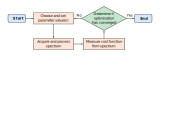
\includegraphics[]{poise/flowchart.png}
    \caption[Flowchart for POISE optimisations]{Flowchart depicting the main steps in a POISE optimisation.}
    \label{fig:poise_flowchart}
\end{figure}

Almost all aspects of this can be customised by the user, which I will now describe.
I make a distinction here between an optimisation \textit{routine}, as well as the \textit{settings} used to run these routines.
Routines consist of a series of predefined variables, such as the parameter(s) to be optimised: however, these may be optimised in different \textit{ways}, which is where the settings come in.
When discussing individual applications in \cref{sec:poise__applications}, I will make repeated reference to these components of an optimisation.

\subsection{Routines}
\label{subsec:poise__routines}

An \textit{optimisation routine}, as defined in POISE, consists of the following components:

\begin{enumerate}
    \item \textit{Name}

        This is an identifier used to refer to the entire routine, which is arbitrary, but should ideally be descriptive.

    \item \textit{Parameters}

        The parameters to be optimised.
        These are given as strings and directly correspond to TopSpin parameter names, for example, \texttt{P1} for a pulse width.

    \item \textit{Initial guess} (one per parameter)

        The point at which the optimisation is started.
        Naturally, this should represent the user's best guess as to where the optimum lies.
        It is generally sensible to choose unoptimised, `default' values for these.
        
    \item \textit{Lower} and \textit{upper bounds} (one of each per parameter)

        These may be chosen based on a range of values which are `chemically sensible'; alternatively, instrumental specifications may sometimes restrict the range of parameter values which can be explored.

    \item \textit{Tolerances} (one per parameter)

        The tolerance loosely corresponds to the level of accuracy required for the optimisation.
        Of course, setting too large a tolerance will simply yield an imprecise and meaningless result.
        However, there is no point in setting this to be too small (i.e.\ requesting an overly accurate optimum): this increases the time required for convergence, because the value of the cost function evaluated at two points too close together will differ only by noise.
        Furthermore, parameter values cannot be implemented with arbitrary precision on a spectrometer, and the available resolution sets a lower bound for the tolerance (see \cref{subsec:poise__epsi} for a more concrete discussion of this).
        These conditions make it sound as if there is little room for error in choosing the tolerance, but in practice the desired accuracy is often reasonably clear from the context, and it generally suffices to get the order of magnitude correct.

    \item \textit{AU programme}

        The AU programme defined in an optimisation routine is used to acquire and process the spectrum.
        The user may leave this empty, in which case POISE automatically detects the dimensionality of the experiment and performs standard processing steps (Fourier transformation, window multiplication, phase correction, and baseline correction).
        This basic setup is often sufficient for many applications.
        However, the AU programme does allow for almost infinite customisation of the actual spectral measurement: for example, it may call other scripts in TopSpin which create shaped pulses (as shown in \cref{subsec:poise__psyche}).

    \item \textit{Cost function}

        The cost function measures the `badness' of the spectrum thus recorded.
        As in the previous chapter, the optimisation algorithm seeks to minimise this value.
        POISE cost functions must be written in Python 3: this design decision is considered later in \cref{subsec:poise__implementation}.
        For ease of use, several cost functions which cover `typical' optimisation scenarios, such as maximising or minimising signal intensity, come pre-installed with POISE.
        This means that users do not necessarily need to write their own cost function if they are not familiar with Python.
\end{enumerate}

Collectively, a routine is therefore a description of \textit{what is to be optimised}.
POISE allows users to create new routines interactively through a series of dialog boxes.
Alternatively, routines themselves can be created on-the-fly using the \texttt{poise -\phantom{}-create} command: this is useful when some components are not known beforehand, such as if the optimum from a different optimisation is to be used as the initial point in a new one.
However, this is limited to single-parameter routines.

After being created, routines are stored in the human-readable JSON format: they can therefore be modified using any text editor.
Examples of these JSON files are presented in subsequent sections.

\subsection{Optimisation settings and algorithms}
\label{subsec:poise__settings}

Once the user has defined a routine, it can then be run from the TopSpin command line using the command \texttt{poise ROUTINE\_NAME}.
However, the routine itself merely controls what parameters are being optimised: it does not specify what experiment is to be run (i.e.\ the pulse programme), nor any of the other parameters in the experiment.
These must be set by the user, and can most conveniently be stored in a TopSpin parameter set which can simply be loaded before starting the optimisation.
This flexibility means that the same \textit{type} of optimisation may be applied to different pulse sequences without having to create individual routines for each: for example, an experiment to optimise the NOE mixing time (as described in \cref{subsec:poise__noe}) can be run with different versions of the NOESY sequence depending on what is most appropriate.
Likewise, parameters such as the number of scans can be adjusted in order to run optimisations on samples with different concentrations.

Once the experiment parameters have been set up, there are a few more options which control how the optimisation is carried out:

\begin{itemize}
    \item the \texttt{--maxfev} option allows the user to control the maximum number of function evaluations, or in other words, the maximum number of experiments run.
        If the optimisation has not converged after acquiring this many spectra, the best result so far is simply returned.
        This effectively allows the time spent on optimisation to be capped.

    \item the \texttt{--quiet} option silences all output from the optimiser (the best parameters found are stored in the dataset itself after the optimisation ends, and can therefore be retrieved).
        This is useful when a POISE optimisation is to be run under automation.
        
    \item the \texttt{--separate} option allows each function evaluation to be run in a new experiment number, so that the optimisation trajectory can be analysed after its conclusion.

    \item perhaps most importantly, the \texttt{--algorithm} option allows the user to choose one of three optimisation algorithms: the \acf{nm} method\autocite{Nelder1965TCJ}, the \acf{mds} method\autocite{Torczon1989,DennisJr1991SIAMJO}, and the Py-BOBYQA trust region method\autocite{Powell2009Proc,Cartis2019ACMTMS}.
        All of these are derivative-free algorithms in that they do not use the value of $\nabla f$ at any point: as described in \cref{subsec:pureshift__optim_techniques}, gradients cannot be accurately estimated when there is noise in the cost function.%
        \footnote{Nocedal and Wright\autocite{Nocedal2006} give an upper bound on the finite difference gradient (as compared to the true gradient) of $\eta(x;\varepsilon)/\varepsilon + O(\varepsilon^2)$, where $x$ is the point at which the gradient is being measured, $\varepsilon$ is the step size used for the finite difference calculation, and $\eta(x;\varepsilon)$ is the noise in the region $[x - \varepsilon, x + \varepsilon]$. If $\varepsilon$ is small, the first term (the error due to noise) is large, and if $\varepsilon$ is large, the second term (the error due to the finite difference approximation) is large.}
        I will now describe these algorithms in slightly greater detail.
\end{itemize}

The NM method is a highly popular derivative-free optimisation algorithm, which maintains a set of points $\{y_1, y_2, \cdots, y_{n+1}\}$ during the optimisation, where $n$ is the number of parameters being optimised.
The convex hull of these points, $Y$, is the smallest possible set of points containing all the $y_k$ such that
\begin{equation}
    \label{eq:convex_hull}
    \forall x_1, x_2 \in Y, \forall \alpha \in [0, 1], \alpha x_1 + (1 - \alpha) x_2 \in Y,
\end{equation}
and is called a \textit{simplex}.
To provide an analogy for $n = 2$, the convex hull is the shape obtained by stretching a rubber band around three pins placed at $y_1, y_2, y_3$.
If this convex hull is nonempty---or equivalently, if the $n$ vectors $y_k - y_1$ ($2 \leq k \leq n + 1$) are linearly independent---then the simplex is called \textit{nonsingular}.
(In the $n = 2$ case, the convex hull would be empty if the three points were collinear.)

\begin{figure}[htb]
    \centering
    
\includegraphics[draft=false]{poise/neldermead.png}
    \caption[Trial points in an iteration of the Nelder--Mead algorithm]{
        Diagram showing various points evaluated in one iteration of the Nelder--Mead algorithm (for an optimisation of two parameters).
        The solid black lines indicate the current simplex, which is assumed to be ordered such that $y_1$ is the best point (has the lowest cost function value) and $y_3$ the worst.
        The blue dots indicate the trial points which the algorithm attempts to replace $y_3$ with, and are further discussed in the text.
        Blue dashed lines indicate the simplex which would result if the corresponding trial point is accepted.
    }
    \label{fig:neldermead}
\end{figure}

The NM algorithm is in fact quite intuitive to understand.
The optimisation begins by measuring the cost function $f$ at every point of the simplex, and sorting the points in ascending order of cost function values (i.e.\ from best to worst), such that $f(y_1) \leq f(y_2) \leq \cdots \leq f(y_{n+1})$.
The centroid of the simplex is defined by the best $n$ points,
\begin{equation}
    \label{eq:simplex_centroid}
    \bar{y} = \sum_{i=1}^n y_i.
\end{equation}
On each iteration of the NM algorithm, we attempt to replace the worst point $y_{n+1}$  with a better point (\cref{fig:neldermead}).
The search for the new point is performed in several steps: first, the worst point is \textit{reflected} about the centroid of the simplex to obtain a new point:
\begin{equation}
    \label{eq:nm_reflect}
    y_\text{r} = \bar{y} - (y_{n+1} - \bar{y}).
\end{equation}
The value of the cost function is evaluated at this point, and is critical in determining how the algorithm proceeds.
If this reflected point falls in the middle of the pack, such that $f(y_1) \leq f(y_\text{r}) < f(y_n)$, this represents a `modest' improvement in the cost function: we simply replace the worst point with this and continue to the next iteration.

On the other hand, if the reflected point is better than all the other points (i.e.\ $f(y_\text{r}) < f(y_1)$), then we ambitiously attempt to \textit{expand} the simplex even further in that direction:
\begin{equation}
    \label{eq:nm_expand}
    y_\text{e} = \bar{y} - 2(y_{n+1} - \bar{y}).
\end{equation}
Of course, there is no guarantee that this is necessarily better than $y_\text{r}$; therefore, we choose whichever point of $y_\text{r}$ or $y_\text{e}$ had a lower value of $f$, and replace the worst point with this and continue to the next iteration.

If the reflected point is an improvement on the worst point but is no better than the remaining points, in that $f(y_n) \leq f(y_\text{r}) < f(y_{n+1})$, then the algorithm performs an \textit{outside contraction}, which resembles a half-hearted reflection:
\begin{equation}
    \label{eq:nm_outside_contract}
    y_\text{oc} = \bar{y} - (1/2)(y_{n+1} - \bar{y}).
\end{equation}
Conversely, if the reflected point is even worse than the worst point ($f(y_{n+1}) \leq f(y_\text{r})$), then this suggests that that search direction is very poor: we thus perform an \textit{inside contraction}, which uses a point halfway between the worst point and the centroid:
\begin{equation}
    \label{eq:nm_inside_contract}
    y_\text{oc} = \bar{y} + (1/2)(y_{n+1} - \bar{y}).
\end{equation}
If either of these contracted points are any better than $y_\text{r}$, then we replace the worst point in the simplex and continue to the next iteration; otherwise, we conclude that no search direction was good, and simply shrink the simplex towards the current best point by replacing each point $y_k$ with $(y_k + y_1)/2$.
In practice, these `last-resort' shrink steps occur very rarely.

\todo{Convergence... self implementation instead of using scipy}

In the preceding discussion, we noted that the simplex $Y$ was nonsingular if the $n$ vectors $y_k - y_1$ were linearly independent.
Equivalently, the matrix $M$ formed by concatenating these vectors
\begin{equation}
    \label{eq:simplex_matrix}
    M = \begin{pmatrix}
        y_2 - y_1, y_3 - y_1, \cdots, y_{n+1} - y_1 \\
    \end{pmatrix}
\end{equation}
must be nonsingular, i.e.\ have a nonzero determinant.
We can quantify how `close' the simplex $Y$ is to being singular, using the $l^2$ condition number of the matrix $M$, which in this context is usually referred to as the \textit{simplex condition}:
\begin{equation}
    \label{eq:simplex_condition}
    \kappa(Y) = \lVert M \rVert \lVert M^{-1} \rVert,
\end{equation}
where $\lVert M \rVert$ is the matrix norm induced by the Euclidean norm,
\begin{equation}
    \label{eq:matrix_norm}
    \lVert M \rVert = \max_{x \neq 0} \frac{\lVert Mx \rVert}{\lVert x \rVert}.
\end{equation}
A singular simplex $Y$ of course does not have a well-defined condition, since $M^{-1}$ does not exist.
However, the larger the condition of a simplex is, the closer it is to being singular.
Very loosely speaking, a long and thin simplex has a large condition number, and would be singular if its width were to go to zero.

The simplex updates made in the process of the NM algorithm mean that the simplex condition changes throughout the course of the optimisation.
If the simplex condition gets too large, it is possible that the optimisation will stall at a nonstationary point, since the search directions of the simplex are severely limited.
The MDS algorithm was proposed partially for the purpose of avoiding this ill-conditioning.\footnote{The main reason was in fact to better exploit computer parallelism, but it was also noticed that the MDS method proved to be generally more robust than NM.}
The MDS method is also simplex-based, but instead of reflecting a single worst point $y_{n+1}$ about the other points, it reflects all of the $n$ worst points $\{y_2, y_3, \cdots, y_{n+1}\}$ about the best point $y_1$.
This means that the shape of the simplex, and thus its condition number, is always preserved; from this, it could be concluded that at least one of the search directions was bounded away from being orthogonal to the gradient.\autocite{Torczon1989}
In simpler terms, at least one of the search directions is `good enough'.

\subsection{Optimisation algorithms}
\label{subsec:poise__algorithms}

As was briefly mentioned in \cref{subsec:pureshift__optim_techniques}, derivative-based optimisation algorithms cannot be used for experimental optimisations.
To be more precise, when analytical gradients are not available, derivative-based algorithms calculate gradients using a finite difference approximation:
\begin{equation}
    \label{eq:finite_difference_grad}
    \nabla f(x) \approx \frac{f(x + \varepsilon) - f(x - \varepsilon)}{2\varepsilon},
\end{equation}
where $\varepsilon$ is the step size used for the finite difference calculation.
In Nocedal and Wright\autocite{Nocedal2006}, it is shown that the error in this finite difference gradient (as compared to the true gradient) has an upper bound of
\begin{equation}
    \label{eq:finite_difference_error}
    \frac{\eta(x;\varepsilon)}{\varepsilon} + O(\varepsilon^2),
\end{equation}
where $\eta(x;\varepsilon)$ is the noise in the region $[x - \varepsilon, x + \varepsilon]$.
If $\varepsilon$ is small, the first term (the error due to noise) is large, and if $\varepsilon$ is large, the second term (which is the error due to the finite difference approximation) is large.
This means that finite difference gradients, and any algorithms which use them, are entirely unreliable in the presence of (sufficient) noise.
Instead, POISE provides a choice of three derivative-free optimisation algorithms: the \acf{nm} method\autocite{Nelder1965TCJ}, the \acf{mds} method\autocite{Torczon1989,DennisJr1991SIAMJO}, and the Py-BOBYQA trust-region method\autocite{Powell2009Proc,Cartis2019ACMTMS}.


\subsubsection{Nelder--Mead}

The NM method is a highly popular derivative-free optimisation algorithm, which maintains a set of points $\{y_1, y_2, \cdots, y_{n+1}\}$ during the optimisation, where $n$ is the number of parameters being optimised.
The convex hull of these points, $Y$, is the smallest possible set of points containing all the $y_k$ such that
\begin{equation}
    \label{eq:convex_hull}
    \forall x_1, x_2 \in Y, \forall \alpha \in [0, 1], \alpha x_1 + (1 - \alpha) x_2 \in Y,
\end{equation}
and is called a \textit{simplex}.
To provide an analogy for $n = 2$, the convex hull is the shape obtained by stretching a rubber band around three pins placed at $y_1, y_2, y_3$.
If this convex hull is nonempty---or equivalently, if the $n$ vectors $y_k - y_1$ ($2 \leq k \leq n + 1$) are linearly independent---then the simplex is called \textit{nonsingular}.
(In the $n = 2$ case, the convex hull would be empty if the three points were collinear.)

\begin{figure}[htb]
    \centering
    
\includegraphics[]{poise/neldermead.png}
    \caption[Trial points in an iteration of the Nelder--Mead algorithm]{
        Diagram showing various points evaluated in one iteration of the Nelder--Mead algorithm (for an optimisation of two parameters).
        The solid black lines indicate the current simplex, which is assumed to be ordered such that $y_1$ is the best point (has the lowest cost function value) and $y_3$ the worst.
        The blue dots indicate the trial points which the algorithm attempts to replace $y_3$ with, and are further discussed in the text.
        Blue dashed lines indicate the simplex which would result if the corresponding trial point is accepted.
    }
    \label{fig:neldermead}
\end{figure}

The NM algorithm is in fact quite intuitive to understand.
The initial simplex is first constructed using the supplied initial point: POISE specifically uses the method of Spendley et al.\autocite{Spendley1962T}
The optimisation itself begins by measuring the cost function $f$ at every point of the simplex, and sorting the points in ascending order of cost function values (i.e.\ from best to worst), such that $f(y_1) \leq f(y_2) \leq \cdots \leq f(y_{n+1})$.
The centroid of the simplex is defined by the best $n$ points,
\begin{equation}
    \label{eq:simplex_centroid}
    \bar{y} = \sum_{i=1}^n y_i.
\end{equation}
On each iteration of the NM algorithm, we attempt to replace the worst point $y_{n+1}$  with a better point (\cref{fig:neldermead}).
The search for the new point is performed in several steps: first, the worst point is \textit{reflected} about the centroid of the simplex to obtain a new point:
\begin{equation}
    \label{eq:nm_reflect}
    y_\text{r} = \bar{y} - (y_{n+1} - \bar{y}).
\end{equation}
The value of the cost function is evaluated at this point, and is critical in determining how the algorithm proceeds.
If this reflected point falls in the middle of the pack, such that $f(y_1) \leq f(y_\text{r}) < f(y_n)$, this represents a `modest' improvement in the cost function: we simply replace the worst point with this and continue to the next iteration.

On the other hand, if the reflected point is better than all the other points (i.e.\ $f(y_\text{r}) < f(y_1)$), then we ambitiously attempt to \textit{expand} the simplex even further in that direction:
\begin{equation}
    \label{eq:nm_expand}
    y_\text{e} = \bar{y} - 2(y_{n+1} - \bar{y}).
\end{equation}
Of course, there is no guarantee that this is necessarily better than $y_\text{r}$; therefore, we choose whichever point of $y_\text{r}$ or $y_\text{e}$ had a lower value of $f$, and replace the worst point with this and continue to the next iteration.

If the reflected point is an improvement on the worst point but is no better than the remaining points, in that $f(y_n) \leq f(y_\text{r}) < f(y_{n+1})$, then the algorithm performs an \textit{outside contraction}, which resembles a half-hearted reflection:
\begin{equation}
    \label{eq:nm_outside_contract}
    y_\text{oc} = \bar{y} - (1/2)(y_{n+1} - \bar{y}).
\end{equation}
Conversely, if the reflected point is even worse than the worst point ($f(y_{n+1}) \leq f(y_\text{r})$), then this suggests that that search direction is very poor: we thus perform an \textit{inside contraction}, which uses a point halfway between the worst point and the centroid:
\begin{equation}
    \label{eq:nm_inside_contract}
    y_\text{oc} = \bar{y} + (1/2)(y_{n+1} - \bar{y}).
\end{equation}
If either of these contracted points are any better than $y_\text{r}$, then we replace the worst point in the simplex and continue to the next iteration; otherwise, we conclude that no search direction was good, and simply shrink the simplex towards the current best point by replacing each point $y_k$ with $(y_k + y_1)/2$.
In practice, these `last-resort' shrink steps occur very rarely.

Finally, convergence is signalled when for each dimension of the optimisation, the width of the simplex is smaller than the chosen optimisation tolerance.%
\footnote{The implementation of the NM algorithm in the \texttt{scipy} library only accepts a single value for the `tolerance', which is then used in all dimensions.
This is designed to be used by scaling the parameters beforehand such that the tolerance in each dimension is equal (and in fact, POISE was later updated to do so).
However, during initial development I chose instead to re-implement the NM algorithm with a convergence check which allowed for different tolerances to be specified in each dimension.}
For a multiple-parameter optimisation, this can potentially mean that extra accuracy is obtained in one of the parameters (because the simplex may have shrunk along that dimension more quickly).
However, it does guarantee that \textit{at least} the specified level of accuracy in every dimension is achieved.


\subsubsection{Multidirectional search}

In the preceding discussion, we noted that the simplex $Y$ was nonsingular if the $n$ vectors $y_k - y_1$ were linearly independent.
Equivalently, the matrix $M$ formed by concatenating these vectors
\begin{equation}
    \label{eq:simplex_matrix}
    M = \begin{pmatrix}
        y_2 - y_1, y_3 - y_1, \cdots, y_{n+1} - y_1 \\
    \end{pmatrix}
\end{equation}
must be nonsingular, i.e.\ have a nonzero determinant.
We can quantify how `close' the simplex $Y$ is to being singular, using the $l^2$ condition number of the matrix $M$, which in this context is usually referred to as the \textit{simplex condition}:
\begin{equation}
    \label{eq:simplex_condition}
    \kappa(Y) = \lVert M \rVert \lVert M^{-1} \rVert,
\end{equation}
where $\lVert M \rVert$ is the matrix norm induced by the Euclidean norm,
\begin{equation}
    \label{eq:matrix_norm}
    \lVert M \rVert = \max_{x \neq 0} \frac{\lVert Mx \rVert}{\lVert x \rVert}.
\end{equation}
A singular simplex $Y$ of course does not have a well-defined condition, since $M^{-1}$ does not exist.
However, the larger the condition of a simplex is, the closer it is to being singular.
Very loosely speaking, a long and thin simplex has a large condition number, and would be singular if its width were to go to zero.

The simplex updates made in the process of the NM algorithm mean that the simplex condition changes throughout the course of the optimisation.
This is good for achieving decreases in the cost function, since the simplex shape \textit{adapts} to the cost function being optimised.
However, if the simplex condition gets too large, it is possible that the optimisation will stall at a nonstationary point, since the search directions of the simplex are severely limited.
The MDS algorithm was proposed partially for the purpose of avoiding this ill-conditioning.\footnote{The main reason was in fact to better exploit computer parallelism, but it was also noticed that the MDS method proved to be generally more robust than NM.}
The MDS method is also simplex-based, and uses similar reflection/expansion/contraction steps as NM.
However, instead of (e.g.) reflecting a single worst point $y_{n+1}$ about the other points, it reflects all of the $n$ worst points $\{y_2, y_3, \cdots, y_{n+1}\}$ about the best point $y_1$.
This means that the shape of the simplex, and thus its condition number, is always preserved, which provides it with much better convergence properties\autocite{Torczon1989,Torczon1991SIAMJO}.%
\footnote{Specifically, it can be concluded that at least one of the search directions was bounded away from being orthogonal to the gradient; or in simpler (and less precise) terms, at least one of the search directions is close enough to a direction in which the cost function $f$ decreases.}

The increased reliability of the MDS algorithm over the NM algorithm was demonstrated on a variety of example optimisation problems: even in the very simple case where the cost function was simply the norm of a vector,
\begin{equation}
    \label{eq:norm_cf}
    f(y) = \lVert y \rVert,
\end{equation}
it was shown that the NM algorithm stalled when the dimension of the problem, $n$, was sufficiently large.
The value of $n$ needed to precipitate this failure depended on the problem being solved, and generally ranged from 8 to 40.
On the other hand, the MDS method proved to be robust under the same conditions, eventually converging to the optimum---although in the cases where NM \textit{did} work, the MDS method generally required more FEs.

It was this improved robustness of the MDS algorithm which prompted Goodwin et al.\autocite{Goodwin2018JMR} to use it in their (experimental) optimisation of ESR pulse shapes, and for me to later include it in POISE.
In the ESR work, the number of pulse points being optimised was 11 or 21, which fell into the regime where the MDS method would likely have better convergence properties than NM.
However, optimisations of this scale are feasible in ESR only because of the rapid relaxation and thus short experiment repetition times.
In NMR, each experiment takes a substantially longer time, and even optimisations with $n > 2$ become rather time-consuming due to the number of FEs required (the largest $n$ explored in the present work is 4).
As will be shown later, we found that the NM and MDS methods were equally reliable in our optimisations, with NM generally being faster.


\subsubsection{Py-BOBYQA}

Unlike the NM and MDS algorithm, Py-BOBYQA is not simplex-based, but is a trust-region algorithm.\autocite{Powell2009Proc,Cartis2019ACMTMS}
The fundamental idea behind a (derivative-free) trust-region method is to sample the cost function at a set of points $Y$, and construct a model $m$ through interpolation, which matches the cost function at these points:
\begin{equation}
    \label{eq:trust_region_model}
    \forall y \in Y, m(y) = f(y).
\end{equation}
The model at iteration $k$ is labelled $m_k$.
Most trust region methods use a quadratic model, and Py-BOBYQA is no exception.
This can be expressed as:
\begin{equation}
    \label{eq:trust_region_quadratic_model}
    m_k(x_k + p) = c + g^Tp + p^TGp,
\end{equation}
where $G$ is a symmetric matrix and $x_k$ is the centre of the model at iteration $k$ ($x_0$ being the user-specified initial point).
For this model to be fully determined, the set $Y$ must therefore contain $(n+1)(n+2)/2$ points in total.%
\footnote{In a derivative-based trust region method, $g$ and $G$ are determined using information from the gradient and/or Hessian.}

The algorithm maintains a \textit{trust region radius} $\Delta_k$ at each iteration, which is a measure of how reliable the model is.
The initial trust region radius, $\Delta_0$, can be arbitrarily chosen: in the case of POISE, I elected to set $\Delta_0$ to be $10$ times the desired tolerance.
The model $m_k$ is then used to calculate the next step $s_k$, which is obtained by minimising $m_k$ over all points within a radius of $\Delta_k$ from the centre $x_k$ (the \textit{trust region subproblem}):
\begin{equation}
    \label{eq:trust_region_subproblem}
    s_k = \argmin_{\lVert s \rVert \leq \Delta_k} m_k(x_k + s).
\end{equation}
Since $m_k$ is noiseless, this can be done with almost any algorithm: Py-BOBYQA uses a conjugate gradient method.
The (true) cost function is then evaluated at the trial point $x_k + s_k$, and compared against the value predicted by the model.
If the ratio of `actual improvement' to `predicted improvement' is large enough, i.e.
\begin{equation}
    \label{eq:trust_region_threshold}
    r_k = \frac{f(x_k) - f(x_k + s_k)}{m_k(x_k) - m_k(x_k + s_k)} \geq \eta
\end{equation}
for some threshold value $\eta$, then the step $s_k$ is accepted and $x_{k+1}$ is set to $x_k + s_k$, replacing the worst point in $Y$.
Additionally, the trust region radius $\Delta_k$ may be increased so that the next step(s) can be more ambitious.
Conversely, if $r_k < \eta$, then there are one of two possibilities: either the model is poorly conditioned (in that the points in $Y$ are very unevenly distributed), in which case one of the points is replaced and the model recalculataed; or the model is sufficiently well-conditioned, in which case the step is rejected, and $\Delta_k$ is decreased.

Py-BOBYQA goes beyond a standard derivative-free trust-region algorithm in further limiting the rate at which the radius $\Delta_k$ can change (amongst others).
Separately from $\Delta_k$, Py-BOBYQA also maintains a lower bound on the trust region radius $\rho_k$, and on unsuccessful iterations $\Delta_k$ is not allowed to decrease further than $\rho_k$.
This prevents $\Delta_k$ from decreasing too quickly until the algorithm is certain that $Y$ is sufficiently well-conditioned.\autocite{Powell2003MP}
Another critical feature of Py-BOBYQA is the implementation of multiple restarts, which endows it with greater robustness towards noise and also allows it to escape local minima.\autocite{Cartis2019ACMTMS,Cartis2022O}
However, the multiple-restarts feature in Py-BOBYQA was disabled in POISE as this often led to overly long optimisations.%
\footnote{Most mathematics papers on optimisation have no qualms in using hundreds or even thousands of FEs, and it is this context in which Py-BOBYQA outperforms other algorithms. Unfortunately for me, POISE works in an \textit{extremely} restrictive regime where even 50 FEs would be considered very expensive.}

Crucially, Py-BOBYQA differs from the simplex-based methods in that \textit{it cares about the actual value of the cost function}.
In the NM and MDS methods, only the relative ordering of the points in the simplex matters; it makes no difference to the algorithm whether the worst point has a cost function value of 10 or 1000.
However, in Py-BOBYQA, the value of $f$ is used in constructing the model, and thus directly influences the optimisation trajectory.
Although this is beneficial in cases where the underlying cost function is relatively well-behaved (this \textit{probably} means cases where the cost function is well described by a quadratic model\footnote{Of course, because of Taylor's theorem, every non-noisy cost function can be locally described by a quadratic model within a sufficiently small region. However, for meaningful progress to be made with noisy cost functions, the model must be built over a large enough region such that noise becomes less relevant.}), and is reflected in faster convergence rates, it can be problematic for some cost functions.
Py-BOBYQA is set as the default optimiser in POISE, but the user is strongly recommended to try the NM method as a first step when troubleshooting failed optimisations.

\section{Implementation}
\label{sec:poise__implementation}

Behind-the-scenes look at the Python 3 implementation.


\section{Applications}
\label{sec:poise__applications}

\subsection{Pulse width calibration}
\label{subsec:poise__pulsecal}

The first of these applications is the calibration of a \ang{90} \proton{} pulse, which is applicable to virtually every NMR experiment.
Essentially, we seek to determine $\taup$ for which
\begin{equation}
    \label{eq:pw90}
    \taup \omega_1 = \frac{\cpi}{2},
\end{equation}
where the RF amplitude $\omega_1$ is not known \textit{a priori} (it is only indirectly controlled via the power level).
This pulse width is conventionally specified as the \texttt{P1} parameter in TopSpin.

\subsubsection{Optimisation setup}

In theory, performing a pulse--acquire experiment with a perfect \ang{180} or \ang{360} pulse would yield no detectable (i.e.\ transverse) magnetisation, i.e.\ a \textit{null}.
Generally, the \ang{360} null is preferred as it minimises effects due to radiation damping, and also allows a smaller recovery delay to be used.
We can use POISE to search for this by acquiring the spectrum, performing a magnitude-mode calculation, and using the intensity of the resulting spectrum as a cost function:
\begin{equation}
    \label{eq:minabsint}
    f_{\symup{m}\text{inabsint}} = \sum_i |S_i|,
\end{equation}
where (reusing notation from \cref{subsec:pureshift__optim_techniques}) $\symbf{S}$ is the spectrum under consideration represented as a complex-valued vector, and the $i$-th point of the spectrum is $S_i = \sqrt{\symbf{S}_{\text{re},i}^2 + \symbf{S}_{\text{im},i}^2}$.
The label \texttt{minabsint} refers to how this cost function drives the optimisation to \textit{min}imise the \textit{abs}olute \textit{int}ensity of the spectrum.
To show how easily this can be coded in Python 3, an implementation of this is shown in \cref{lst:minabsint} (for all other cost functions in this chapter, the reader is directed to the POISE source code for their implementations).
The \texttt{get1d\_...} helper functions are provided by POISE.

\begin{mylisting}[htb]
\begin{tcbminted}{python}
import numpy as np

def minabsint():
    r = get1d_real()
    i = get1d_imag()
    mag = np.abs(r + 1j * i)
    return np.sum(mag)
\end{tcbminted}
\caption[Implementation of \texttt{minabsint} cost function]{The implementation of the \texttt{minabsint} cost function in POISE.}
\label{lst:minabsint}
\end{mylisting}

\begin{figure}[htb]
    \centering
    \includegraphics[]{poise/p1_scan.png}%
    \caption[Reference grid search for pulse width optimisation]{
        Reference grid search, showing how the \texttt{minabsint} cost function varies with the pulse width \texttt{P1}.
        \datacode{6F-200826}
    }
    \label{fig:p1_scan}
\end{figure}

To check whether this cost function was sensible, I manually acquired a series of spectra with a range of pulse widths and calculated $f_{\symup{m}\text{inabsint}}$ for all of these (\cref{fig:p1_scan}).
In this chapter, I will refer to this process as a \textit{reference grid search}.
It should be noted that reference grid searches are a time-consuming procedure, and an end-user of POISE generally does \textit{not} need to do this (it would defeat the purpose of the optimisation).
I only perform one here to provide some insight into the nature of the optimisation.
In any case, the reference grid search makes it clear that there is a well-defined minimum, located in this case at \qty{48.3}{\us}; if the POISE optimisation process is accurate, it should converge to this point.

I chose the initial point to be four times the \texttt{prosol} value for \texttt{P1}, which evaluates to \qty{48}{\us} for the spectrometer used here: this represents our `best guess' and is derived from prior calibration of the pulse width on a standard sample.
The tolerance is set to \qty{0.2}{\us}, which corresponds to an accuracy of \qty{0.05}{\us} for the \ang{90} pulse width itself.
The lower and upper bounds are set to be \qty{8}{\us} away from the initial point, representing a `sensible' region within which we expect the null to lie (this may need to be adjusted for samples with high ionic strength, but for typical organic samples this is more than enough).
A standard \texttt{poise\_1d} acquisition AU programme is used, which simply acquires the spectrum and performs Fourier transformation, phase correction, and baseline correction.
The routine in JSON format is shown in the caption of \cref{tbl:poisecal_48}.
Finally, in order to reduce the time taken for the optimisation, several tricks are used: each FE is run using no dummy scans and only one scan, the acquisition time is set to just \qty{1.1}{\s} (high resolution is not required for a reliable cost function value), and the recovery delay \texttt{D1} is set to 0.
In practice, there is an extra gap of around \qty{5}{\s} between successive FEs due to spectrometer initialisation, so an extra recovery delay is not needed.


\subsubsection{The competition}

The performance of POISE can be compared against two `competitors' in this area.
The traditional method of determining the \ang{90} pulse width is to measure a pulse width array (colloquially, `to array the pulse width').\autocite{Keifer1999CMR}
This entails measuring a series of pulse--acquire spectra, over which $\taup$ is evenly incremented: in optimisation parlance this would be called a \textit{grid search}.%
\footnote{This differs from the \textit{reference grid search} above only in spirit (hence the similar names). The process is exactly the same, but the grid search is used to actually locate the optimum, whereas in the reference grid search my aim is purely to verify whether the faster optimisation algorithms converge to the correct point.}
This leads to a sinusoidal pattern in the peak intensities, from which the \ang{360} null can be directly read off.
An example of this is shown in \cref{fig:p1_scan_spectra}, where the \ang{360} null at $\taup \approx \qty{48}{\us}$ is visible (it is never a \textit{perfect} null because of off-resonance effects and $\omega_1$, i.e.\ $B_1$, inhomogeneity).

\begin{figure}[htb]
    \centering
    \includegraphics[]{poise/p1_scan_spectra.png}%
    \caption[Pulse width array]{
        An example of a pulse width array, where the variation of the water peak is monitored with changes in pulse width (this sample is in DMSO-$d_6$, but is slightly wet).
        These spectra were acquired manually before plotting; the TopSpin \texttt{popt} command would yield essentially identical results.
        \datacode{6F-200826}
    }
    \label{fig:p1_scan_spectra}
\end{figure}

TopSpin provides a built-in mechanism for measuring a pulse width array using the \texttt{popt} command.
The pulse--acquire spectrum is measured for pulse widths between a lower and upper bound, and the user specifies a spectral region of interest which \texttt{popt} uses to determine the null in spectrum intensity.%
\footnote{In fact, \texttt{popt} uses the notion of a cost function as well, in that it determines the point where the cost function is minimised. In this case, I set it to use the \texttt{MAGMIN} cost function, which seeks to minimise the intensity of the magnitude-mode spectrum; this is essentially identical to the \texttt{minabsint} cost function which was used for the POISE optimisations except that it only applies to the spectral region of interest.}
While this usually yields highly accurate results, the acquisition of so many spectra is relatively time-consuming and arguably unnecessary if the only purpose is to determine the null.

A more rapid method for pulse calibration is the nutation experiment of Wu and Otting\autocite{Wu2005JMR}, which allows the \ang{90} pulse width to be determined in a single-scan experiment.
In this experiment, an RF pulse with a given power level, corresponding to an (unknown) amplitude of $\omega_1'$, is applied during acquisition.%
\footnote{To be precise, it is applied for a proportion $d$ of the dwell time between acquisition of successive points in the FID; $d$ is called the \textit{duty cycle} and must be accounted for when calculating the pulse width using this method.}
Assuming that the pulse is applied along the $x$-axis, this leads to the following product operators during the acquisition period:
\begin{equation}
    \label{eq:pulsecal_operators}
    I_z \xrightarrow{\omega_1' t_2} I_z \cos(\omega_1' t_2) - I_y \sin(\omega_1' t_2)
\end{equation}
and (since we only detect $I_-$) an FID of
\begin{equation}
    \label{eq:pulsecal_signal}
    s(t_2) = \frac{1}{2\mi}\sin(\omega_1't_2) = -\frac{1}{4}[\exp(\mi \omega_1' t_2) - \exp(-\mi \omega_1' t_2)],
\end{equation}
which when Fourier transformed yields an antiphase doublet where the two peaks are separated by the frequency $2\omega_1'$.
Measuring the separation between the two peaks directly yields the unknown amplitude $\omega_1'$, from which $\taup' = \cpi/(2\omega_1')$ can be calculated.
Typically, the RF amplitude $\omega_1'$ is rather smaller than the amplitude $\omega_1$ which we would like to apply the hard pulse at, and thus $\taup' > \taup$.
However, this can be adjusted for using the power levels applied (which are known to the user).

Although the nutation experiment can be performed extremely quickly using the TopSpin \texttt{pulsecal} command, often only requiring a few seconds, the pulse widths calculated are generally slightly shorter compared to the value obtained from a \ang{360} null.
This is a known effect which arises because the separation is calculated from the top of the peaks, which correspond to the most homogeneous region of the $B_1$ profile.\autocite{Wu2005JMR}
On the other hand, the \ang{360} null (as measured through \texttt{popt} or POISE, for example) measures a signal which is averaged over the entire $B_1$ profile.


\subsubsection{Optimisation results}

\begin{table}[!ht]
    \centering
    \begin{tabular}{ccccc}
        \toprule
        Entry & Method & Optimum found (\unit{\us}) & FEs & Time taken (\unit{\s}) \\
        \midrule
        1  & \texttt{popt}      & 48.40        & 41   & 299    \\
        2  & \texttt{pulsecal}  & 46.64        & --   & 37     \\
        3 & POISE (NM)         & 48.38        & 10   & 76--79 \\
        4 & POISE (MDS)        & 48.38        & 10   & 77--80 \\
        5 & POISE (BOBYQA)  & 48.29--48.41 & 6--7 & 46--54 \\
        \bottomrule
    \end{tabular}
    \caption[Comparison of methods for \ang{360} pulse width determination]{
        Comparison of methods for \ang{360} pulse width determination.
        \texttt{popt} grid searches were run between values of \qty{40}{\us} and \qty{56}{\us}, with a linear increment of \qty{0.4}{\us} (which, through interpolation, provides a precision of approximately \qty{0.2}{\us} in the result, matching the tolerance used for POISE).
        \texttt{pulsecal} was run as normal and the reported pulse width multiplied by 4 to obtain the \ang{360} pulse width for comparison.
        POISE optimisations were run according to the routine in \cref{tbl:poisecal_48}.
        \datacode{6F-200826}
    }
    \label{tbl:poisecal_48}
\end{table}

Compared to these two existing methods, we expect POISE to be faster than the \texttt{popt} grid search, and also more accurate than the nutation experiment in \texttt{pulsecal}.
This is borne out in practice (\cref{tbl:poisecal_48}).
\texttt{popt} yields an optimum of \qty{48.4}{\us}, which is closely matched by POISE.
However, across all five optimisation runs performed for each algorithm, POISE locates this optimum using far fewer FEs (and far less time) because its algorithms are more efficient than a simple grid search.
While the \texttt{pulsecal} routine is even faster than POISE,%
\footnote{\texttt{pulsecal} could be yet faster if it was instructed to not optimise the receiver gain prior to performing the nutation experiment.}
it underestimates the \ang{90} pulse width by about 4\%.
In this particular case, POISE is the only option which strikes a useful balance between speed and accuracy.
These results also provide the first evidence that Py-BOBYQA is generally faster than the simplex-based methods: this observation is consistently reproduced in many of the other optimisations in this chapter.


\subsubsection{Different initial points}

One question we might reasonably ask is how robust POISE is towards poor initial guesses.
In the case of the pulse width calibration, the answer is \textit{very} robust.
\Cref{tbl:poisecal_43,tbl:poisecal_53} summarise the results obtained with an initial guess of \qty{43}{\us} and \qty{53}{\us} respectively.
There is slightly decreased performance in that a few more FEs are required for convergence, but the accuracy of the result is unchanged.

\begin{table}[htb]
    \centering
    \begin{tabular}{ccccc}
        \toprule
        Entry & Method      & Optimum found (\unit{\us}) & FEs & Time taken (\unit{\s}) \\
        \midrule
        1 & POISE (NM)     & 48.38        & 14 & 109--114 \\
        2 & POISE (MDS)    & 48.38        & 14 & 108--112  \\
        3 & POISE (BOBYQA) & 48.27--48.33 & 9  & 70       \\
        \bottomrule
    \end{tabular}
    \caption[Pulse width calibrations using initial guess of \qty{43}{\us}]{
        Pulse width optimisations with an initial point of \qty{43}{\us}.
        The POISE routine is the same as in \cref{tbl:poisecal_48}, except with \texttt{"init":[43.0]}.
        \datacode{6F-200826}
    }
    \label{tbl:poisecal_43}
\end{table}

\begin{table}[htb]
    \centering
    \begin{tabular}{ccccc}
        \toprule
        Entry & Method      & Optimum found (\unit{\us}) & FEs & Time taken (\unit{\s}) \\
        \midrule
        1 & POISE (NM)     & 48.38        & 14 & 110--114 \\
        2 & POISE (MDS)    & 48.25--48.38 & 16 & 123--126 \\
        3 & POISE (BOBYQA) & 48.26--48.33 & 9  & 69--70   \\
        \bottomrule
    \end{tabular}
    \caption[Pulse width calibrations using initial guess of \qty{53}{\us}]{
        Pulse width optimisations with an initial point of \qty{53}{\us}.
        The POISE routine is the same as in \cref{tbl:poisecal_48}, except with \texttt{"init":[53.0]}.
        \datacode{6F-200826}
    }
    \label{tbl:poisecal_53}
\end{table}

It is tempting to use this example to draw the conclusion that the initial point does not matter in POISE optimisations.
However, this is only really true for a simple optimisation like this.
Looking again at the reference grid search in \cref{fig:p1_scan}, it is clear that there is no other possible minimum that the optimiser could converge to.
Furthermore, the noise in the cost function is almost indiscernible.
These represent the \textit{ideal} conditions for an experimental optimisation to work, and it is not surprising that extremely good performance is obtained with POISE.
Some of the subsequent examples include more difficult or more noisy cost functions.
We will see that POISE does indeed have \textit{some} tolerance towards poor initial points, even in the presence of noise (after all, this is the entire purpose of using derivative-free algorithms).
However, for very challenging optimisations (especially ones with many parameters) it is very likely that the optimisation will ultimately converge to a local minimum close to the initial point, which may not necessarily yield a substantial reduction in the cost function.

\subsection{Ernst angle optimisation}
\label{subsec:poise__ernst}

Often, in a simple 1D pulse--acquire spectrum it is not hugely important to know the exact \ang{90} pulse width: instead, it is more valuable to optimise the sensitivity per unit time of the spectrum.

\subsubsection{Optimisation setup}

\begin{figure}[htb]
    \centering
    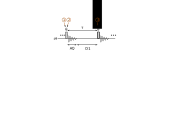
\includegraphics[]{pp/poise/zg_repeated.png}%
    \caption[Steady-state pulse--acquire experiment]{Steady-state pulse--acquire experiment. The excitation flip angle is $\theta$, and the repetition time between experiments is $\taur$.}
    \label{fig:zg_ernst}
\end{figure}

Before launching straight into how this may be obtained through optimisation, it is instructive to first consider which parameters are worth optimising.
For a pulse--acquire experiment (\cref{fig:zg_ernst}), the repetition time is the sum of the acquisition time \texttt{AQ} plus the recovery delay \texttt{D1}; the flip angle $\theta$ is controlled via the pulse width \texttt{P1}.
We assume that the experiment has been repeated enough times to reach a \textit{steady state}, that is, the amount of $z$-magnetisation prior to the excitation pulse (point \circled{1}) is a constant $M_{z,\text{ss}}$.
Application of the excitation pulse leads to a signal scaling as $M_{z,\text{ss}}\sin\theta$, and residual (unexcited) longitudinal magnetisation of $M_{z,\text{ss}}\cos\theta$ at point \circled{2}.
After the repetition time $\taur$ (point \circled{3}), it can be shown using the Bloch equations\autocite{Bloch1946PR} that the $z$-magnetisation recovers to
\begin{equation}
    \label{eq:z_magn_ernst1}
    M_{z,0}(1 - c) + cM_{z,\text{ss}}\cos\theta,
\end{equation}
where $c = \exp(-\taur/T_1)$ and $M_{z,0}$ is the initial, equilibrium $z$-magnetisation (before the experiment begins).
Since the experiment has reached a steady state, points \circled{1} and \circled{3} are equivalent: thus, we have that
\begin{equation}
    \label{eq:z_magn_ernst2}
    M_{z,0}(1 - c) + cM_{z,\text{ss}}\cos\theta = M_{z,\text{ss}},
\end{equation}
which can be rearranged to give
\begin{equation}
    \label{eq:z_magn_ernst3}
    \frac{M_{z,\text{ss}}}{M_{z,0}} = \frac{1 - c}{1 - c\cos\theta}.
\end{equation}
The signal amplitude $s$ therefore scales as
\begin{equation}
    \label{eq:z_magn_ernst4}
    s = \frac{(1 - c)}{1 - c\cos\theta} \cdot \sin\theta,
\end{equation}
and is maximised when $\md s/\md \theta = 0$, the solution of which is the celebrated \textit{Ernst angle}\autocite{Ernst1966RSI}:
\begin{equation}
    \label{eq:ernst_angle}
    \theta_\text{E} = \arccos{c} = \arccos\left[\exp\left(-\frac{\taur}{T_1}\right)\right].
\end{equation}
In general, $T_1$ and hence $\theta_\text{E}$ varies across the different spins in a given sample, so some degree of compromise is required in order to maximise sensitivity for all peaks.

Naively, we may then consider fixing $\taur$ and optimising \texttt{P1} to locate the Ernst angle (or to be precise, the pulse width which corresponds to the Ernst angle, since that is the only quantity we really care about).
This is generally true.
However, we can go one step further, because $\taur$ itself is comprised of two parameters, and the sensitivity \textit{per unit time} may be affected by varying $\taur$.
Since the signal scales as $1/\taur$ (a shorter $\taur$ means more repetitions per unit time) but the noise scales only as $\sqrt{1/\taur}$, the sensitivity per unit time is
\begin{equation}
    \label{eq:z_magn_ernst5}
    S = \frac{(1 - c)\sin\theta}{(1 - c\cos\theta)\sqrt{\taur}}.
\end{equation}
Assuming that $\theta$ is always set to the respective Ernst angle for different $\taur$, it can be shown that the best sensitivity per unit time is attained when $\taur \to 0$.\autocite{Waugh1970JMS,Traficante1992CMR}
Of course, this limit is not physically possible: $\taur$ comprises the acquisition time which must be nonzero.
However, it does imply that \texttt{AQ} should be kept as short as possible, and \texttt{D1} set to zero, as shown in \cref{fig:ernst_sensitivity}.

\begin{figure}[htb]
    \centering
    \includegraphics[]{poise/ernst_sensitivity.png}%
    \caption[Sensitivity per unit time as a function of \texttt{AQ} and \texttt{D1}]{Sensitivity per unit time as a function of \texttt{AQ} and \texttt{D1}, assuming that an Ernst angle excitation pulse is used. $T_1$ was set to \SI{1.5}{\s}.}
    \label{fig:ernst_sensitivity}
\end{figure}

Knowing this, we can then set up a meaningful optimisation routine.
We seek to optimise the pulse width \texttt{P1} such that the intensity of the real part of the spectrum is maximised (corresponding to a \texttt{maxrealint} cost function).
In practice, I took the extra step of calibrating the \ang{90} pulse width (as per the previous section) and modifying the pulse programme such that the flip angle could be specified as the parameter \texttt{CNST20}: this is not generally necessary and is only useful for evaluating the results, as will be shown later.
As per the above analysis, I set \texttt{AQ} and \texttt{D1} to be \SI{1.2}{\s} and 0 respectively.
The number of scans (\texttt{NS}) can be set to 1, but unlike in the pulse width calibration (\cref{subsec:poise__pulsecal}), we must use enough dummy scans to ensure that a steady-state signal intensity is recorded: in practice I set \texttt{DS=4}.
This means that each FE, and thus the overall optimisation, requires a slightly longer time than the pulse width calibrations previously shown.


\subsubsection{Optimisation results}

The Ernst angle optimisation was run with two different spectral regions of interest: firstly, on all the aromatic and olefinic peaks in the sample of ferulic acid (\cref{tbl:poise_ernst_fivepeaks}), and secondly, on only the peak at \SI{6.79}{\ppm} (\cref{tbl:poise_ernst_onepeak}).
(This spectral region can be selected using the TopSpin \texttt{dpl} command, which stores the bounds using the parameters \texttt{F1P} and \texttt{F2P}: all built-in cost functions respect these two parameters.)
Generally, optimisations could be completed in under two minutes.
The optima found for these two optimisations are different: this is because the former searches for a compromise Ernst angle which balances $T_1$ of all peaks within the region, and the latter optimises only for one $T_1$.

\begin{table}[htb]
    \hbadness=10000
    \centering
    \begin{tabular}{ccccc}
        \toprule
        Entry & Algorithm & Optimum found ($^\circ$) & FEs   & Time taken (\si{\s}) \\
        \midrule
        1     & NM        & 67.5--73.1               & 9--13 & 91--132              \\
        2     & MDS       & 67.5--73.1               & 9     & 90--92               \\
        3     & BOBYQA    & 70.1--70.7               & 7     & 70--71               \\
        \bottomrule
    \end{tabular}
    \caption[Ernst angle optimisations on a range of peaks]{
        Ernst angle optimisation, performed on all aromatic and olefinic peaks in ferulic acid (between 6 and \SI{8}{\ppm}).
        The POISE routine used here is: \mintinline[breaklines]{json}{{"name": "ernst", "pars": ["cnst20"], "lb": [10.0], "ub": [90.0], "init": [30.0], "tol": [3.0], "cf": "maxrealint", "au": "poise_1d"}}.
        \datacode{5F-210619}
    }
    \label{tbl:poise_ernst_fivepeaks}
\end{table}

\begin{table}[htb]
    \hbadness=10000
    \centering
    \begin{tabular}{ccccc}
        \toprule
        Entry & Algorithm & Optimum found ($^\circ$) & FEs   & Time taken (\si{\s}) \\
        \midrule
        1     & NM        & 60.0--67.5               & 9--11 & 91--111              \\
        2     & MDS       & 65.6--67.5               & 11    & 110--111             \\
        3     & BOBYQA    & 60.0--65.2               & 6--7  & 59--71               \\
        \bottomrule
    \end{tabular}
    \caption[Ernst angle optimisations on only one peak]{
        Ernst angle optimisations on the peak at \SI{6.79}{\ppm} in ferulic acid.
        The POISE routine is the same as in \cref{tbl:poise_ernst_fivepeaks}, but the spectral region under optimisation was set to be 6.71--\SI{6.87}{\ppm}
        The theoretical optimum, as given in \cref{tbl:ernst_invrec}, is \ang{61.6}.
        \datacode{5F-210619}
    }
    \label{tbl:poise_ernst_onepeak}
\end{table}

To determine the accuracy of the optima found, rather than performing a reference grid search as in \cref{subsec:poise__pulsecal}, I measured $T_1$ of each of these peaks using a typical gradient-enhanced inversion--recovery experiment, and calculated the theoretical Ernst angles from this (\cref{tbl:ernst_invrec}).
The first optimisation, which should yield essentially a weighted average of the five Ernst angles, appears at first glance to be biased towards larger values.
However, this can be rationalised by the fact that that a flip angle larger than $\theta_\text{E}$ is less detrimental to sensitivity compared to one that is smaller (this can be seen by plotting \cref{eq:z_magn_ernst4}).
On the other hand, the second optimisation yields an accurate value for the relevant peak (number 4 in \cref{tbl:ernst_invrec}), at least to within the specified tolerance of \ang{3}.

\begin{table}[htb]
    \centering
    \begin{tabular}{ccccc}
        \toprule
        Peak & \proton{} chemical shift (ppm) & $T_1$ (\si{\s}) & $\theta_\text{E}$ ($^\circ$) & $T_1\ln 2$ (\si{\s})\\
        \midrule
        1 & 7.49 & 1.750 & 59.8 & 1.213 \\
        2 & 7.27 & 0.977 & 73.0 & 0.677 \\
        3 & 7.08 & 1.279 & 67.0 & 0.887 \\
        4 & 6.79 & 1.615 & 61.6 & 1.119 \\
        5 & 6.36 & 1.415 & 64.6 & 0.981 \\
        \bottomrule
    \end{tabular}
    \caption[$T_1$ values for ferulic acid]{
        $T_1$ and corresponding Ernst angles for each peak in ferulic acid, calculated for a repetition time of \SI{1.20}{\s}.
        The values of $T_1 \ln 2$ are also provided here, in anticipation of the inversion--recovery experiments performed in \cref{subsec:poise__invrec}.
        \datacode{5F-210619}
    }
    \label{tbl:ernst_invrec}
\end{table}

Finally, it is worth considering whether this optimisation is truly worth it.
\proton{} pulse--acquire spectra already have a very high intrinsic sensitivity, and in the two minutes taken to optimise the flip angle, one could easily just acquire (around) 64 more scans, at which point knowledge of the Ernst angle would cease to be useful.
It \textit{may} be more useful for nuclei which have lower sensitivity, such as \carbon{}: I did not evaluate this possibility.
However, it must be borne in mind that a low-sensitivity experiment will also require more scans per FE, which leads to a corresponding increase in the optimisation time.

In my estimation, a more useful application of this optimisation routine would be to use it to determine an average $T_1$ value for a group of peaks.
This could then be used to inform the choice of recovery delay for multidimensional experiments\autocite{Reynolds2002JNP,Burns2021MRC} or quantitative NMR experiments\autocite{Pauli2005JNP,Giraudeau2014MRC}.
It is, however, possible to more directly obtain $T_1$ values from an inversion--recovery experiment, which I describe next.

\subsection{NOE mixing time}
\label{subsec:poise__noe}

Stuff

\subsection{ASAP-HSQC excitation delay}
\label{subsec:poise__asaphsqc}

INEPT

\subsection{HMBC low-pass J-filter}

Artefacts.

\subsection{Inversion--recovery}
\label{subsec:poise__invrec}

Stuff

\subsection{Ultrafast NMR}

EPSI gradient imbalance

\subsection{PSYCHE pure shift NMR}
\label{subsec:poise__psyche}

In \cref{sec:pureshift__optimisation}, I described early attempts towards the optimisation of PSYCHE pure shift spectra.
The content in this section is similar, except that it was performed within the framework of POISE.

\begin{figure}[htb]
    \centering
    
\includegraphics[]{pp/poise/psyche.png}
    {\phantomsubcaption\label{fig:poise_psyche_pulseq_psyche}}
    {\phantomsubcaption\label{fig:poise_psyche_pulseq_jrse}}
    \caption[Pulse sequences used for PSYCHE optimisations]{
        \textbf{(\subref{fig:poise_psyche_pulseq_psyche})} Pseudo-2D PSYCHE pure shift experiment.
        \textbf{(\subref{fig:poise_psyche_pulseq_jrse})} J-resolved spin echo experiment (see also \cref{subsec:pureshift__optim_techniques}) using the PSYCHE PSE.
        Phase cycling is performed using: $\phi_1 = (x, -x)$, $\phi_2 = (x, x, y, y)$, $\phi_{\text{rec},1} = (x, -x, -x, x)$ for the full PSYCHE experiment, and $\phi_3 = (x, y, -x, -y)$, $\phi_{\text{rec},2} = (x, -x, x, -x)$ for the JRSE experiment.
        Gradient amplitudes are $(g_1, g_2, g_3, g_4) = (35\%, 77\%, 2\%, 50\%)$ (though the exact value of the CTP gradients are likely immaterial).
        The delay $\tau$ is set to $1/(4 \cdot T_\text{chunk})$ for the PSYCHE experiment, and $\tau_\text{e}$ is \SI{16}{\ms}.
    }
    \label{fig:poise_psyche_pulseq}
\end{figure}



\subsubsection{Optimisation setup}

In this section, the standard double-saltire PSYCHE pure shift element was used (\cref{fig:poise_psyche_pulseq_psyche}).
As described in \cref{subsec:pureshift__optim_techniques}, the PSYCHE pure shift element can be described using six parameters; in this section, we investigate only three of these, namely the amplitude (i.e.\ flip angle), bandwidth, and duration.
In addition to this, the amplitude of the weak gradient during the PSE was also chosen as a fourth parameter to vary.
As before, the quality of the PSE is evaluated using a JRSE experiment (\cref{fig:poise_psyche_pulseq_jrse}), which is then compared against a pulse--acquire spectrum: the cost function used is $f_\text{diff}$.
In general, the spectral region being evaluated has to be appropriately chosen to exclude strong singlets, which are irrelevant to pure shift NMR but disproportionately influence the value of the cost function.


\subsection{Solvent suppression}
\label{subsec:poise__solvsupp}

Mouse

\subsection{Diffusion NMR}
\label{subsec:poise__diffusion}

As the final example of a POISE optimisation, I demonstrate its application to \acf{dosy} experiments.\autocite{Johnson1999PNMRS}
DOSY experiments measure molecular diffusion during a delay period, $\Delta$, which is placed between two gradients, such as in the stimulated echo experiment (\cref{fig:poise_dosy_pulseq_ste}), or the bipolar pulse pair version (\cref{fig:poise_dosy_pulseq_stebpp}) which uses opposing gradients to refocus the lock signal during the sequence.
In these sequences, the first `encoding' gradient (or set thereof) imparts a spatially-dependent phase, which---in the absence of diffusion---is perfectly refocused by the second `decoding' gradient (or set thereof).
However, if diffusion is present, this refocusing is not complete, leading to signal attenuation which is described by the Stejskal--Tanner equation:
\begin{equation}
    \label{eq:stejskal_tanner_again}
    I(G) = I(0) \exp\left[-(\gamma\delta G)^2 D \Delta'\right].
\end{equation}
Here, $G$ is the amplitude of the encoding and decoding gradients, $\delta$ the duration of the gradients, and $\Delta'$ is a corrected diffusion delay.

\begin{figure}[htb]
    \centering
    
\includegraphics[]{pp/poise/dosy.png}
    {\phantomsubcaption\label{fig:poise_dosy_pulseq_ste}}
    {\phantomsubcaption\label{fig:poise_dosy_pulseq_stebpp}}
    {\phantomsubcaption\label{fig:poise_dosy_pulseq_oneshot}}
    \caption[Selection of DOSY pulse sequences]{
        \textbf{(\subref{fig:poise_dosy_pulseq_ste})} Stimulated echo DOSY pulse sequence. The diffusion-encoding and -decoding gradients, whose amplitudes are incremented, are marked with arrows.
        \textbf{(\subref{fig:poise_dosy_pulseq_stebpp})} Stimulated echo bipolar pulse pair DOSY pulse sequence.
        \textbf{(\subref{fig:poise_dosy_pulseq_oneshot})} Oneshot DOSY pulse sequence.
    }
    \label{fig:poise_dosy_pulseq}
\end{figure}

In a 2D DOSY experiment, each increment is recorded with a different gradient amplitude $G$.
The value of $D$ can then be extracted through various means, most simply an exponential fitting of the measured intensities $I(G)$ for single species (or distinct species which do not overlap).
In order to minimise the uncertainty in the calculated diffusion coefficients, the parameters $\Delta$ and $\delta$, as well as the range of gradient amplitudes used (and possibly also their distribution), should be chosen in order to yield a diffusion profile of the form in \cref{fig:diffusion_sim_ok}.
Generally, the last increment (acquired using the maximum gradient strength, $G_\text{max}$ should have an attenuation of 5--35\%\footnote{Recommendations tend to vary.} when compared against the first increment (acquired with the minimum gradient amplitude, $G_\text{min}$, which may be 0).
Traditionally, this is done `by hand' by acquiring individual increments of the 2D diffusion experiment, checking the attenuation, and adjusting the parameters accordingly.\autocite{Johnson1999PNMRS,Claridge2016}

\begin{figure}[htb]
    \centering
    \includegraphics[]{poise/diffusion_sim.png}%
    {\phantomsubcaption\label{fig:diffusion_sim_weak}}%
    {\phantomsubcaption\label{fig:diffusion_sim_ok}}%
    {\phantomsubcaption\label{fig:diffusion_sim_strong}}%
    \caption[Simulated diffusion profiles for slow, intermediate, and rapid diffusion]{
        Simulated diffusion profiles for species with different diffusion rates.
        \textbf{(\subref{fig:diffusion_sim_weak})} A slowly diffusing species: insufficient attenuation is observed with the given parameters, meaning that generally $\Delta$ or $\delta$ need to be increased.
        \textbf{(\subref{fig:diffusion_sim_ok})} An `ideal' diffusion profile where attenuation is neither too little or too much.
        \textbf{(\subref{fig:diffusion_sim_strong})} A rapidly diffusing species, for which complete attenuation is already accomplished using low gradient amplitudes. This generally suggests that $\Delta$ or $\delta$ need to be decreased, or a new gradient ramp calculated.
    }
    \label{fig:diffusion_sim}
\end{figure}

This task could of course be delegated to a computer programme such as POISE.
We \textit{could} simply tackle it head-on by optimising all of $\Delta$, $\delta$, and $G_\text{max}$ at once (assuming that $G_\text{min}$ is fixed); however, this is actually rather inefficient.
Firstly, we previously saw that multiple-parameter optimisations took a longer time than the corresponding single-parameter optimisations.
However, on top of that, it is often not even necessary to change all three parameters: the Stejskal--Tanner equation shows that the diffusion attenuation is controlled only by the overall \textit{product} $\delta^2 G_\text{max}^2 \Delta'$.
Thus, at least to a first approximation, the individual values of $\Delta$, $\delta$, and $G_\text{max}$ do not actually matter.
It makes sense to fix two of these and optimise one parameter, only changing the other two if necessary.

It should be mentioned here that obtaining \textit{accurate} values of $D$ requires careful consideration of various factors such as the exact DOSY sequence and gradient shapes used\autocite{Sinnaeve2012CMR}, peak overlap\autocite{Antalek1996JACS,Windig1997CILS,Nilsson2006AC,Nilsson2008AC,Colbourne2011JACS}, and convection\autocite{Swan2015JMR,Barbosa2016RSCA}.
This may influence the type of processing which is chosen for extraction of diffusion coefficients.
However, these issues are not our concern here: the role of POISE is only to find a good set of acquisition parameters such that the resulting data is amenable towards further processing.


\subsubsection{Optimisation setup}

The overall strategy for this `optimisation' can be briefly summarised in a flowchart (\cref{fig:dosy_flowchart}).
Note that this is \textit{not} a classic optimisation which falls nicely into the POISE workflow (\cref{fig:poise_flowchart}): thus, the entire procedure cannot simply be summarised into one POISE routine.
However, it does contain two optimisation subproblems: one to adjust $\Delta$ if necessary, and one to find $G_\text{max}$.
We can therefore create a wrapper script for the overall procedure (here called \texttt{dosy\_opt.py}, which invokes POISE to solve the two individual subproblems.
This approach is made possible by the command-line interface of POISE, which allows for the creation and execution of optimisation routines.
We also exploit the fact that during the optimisation, POISE stores the value of the cost function as the \texttt{TI} parameter in TopSpin.
This fact is often irrelevant as the value of the cost function is not often of great interest, but proves to be handy in this particular instance as it allows POISE to pass information back to the wrapper script.
Previously, we explored situations where the functionality of POISE could be extended from \textit{within}, e.g.\ by invoking different scripts in its acquisition AU programme.
In this case, we are going in the other direction, allowing POISE to be incorporated in other scripts.

\begin{figure}[htb]
    \centering
    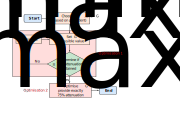
\includegraphics[]{poise/dosy_flowchart.png}%
    \caption[Flowchart for DOSY parameter optimisation]{
        Flowchart for DOSY parameter optimisation. In fact, this consists of two subproblems which can be individually solved using POISE.
    }
    \label{fig:dosy_flowchart}
\end{figure}

The DOSY optimisation procedure uses a 1D pulse programme throughout: this should essentially be a single increment of the desired 2D DOSY experiment.%
\footnote{1D versions of most DOSY variants are available in the TopSpin standard library, but can also be easily obtained by disabling the gradient incrementation in the 2D versions.}
In this work, I specifically used the Oneshot DOSY sequence\autocite{Pelta2002MRC} (\cref{fig:poise_dosy_pulseq_oneshot}): this sequence has the advantage of not requiring onerously long phase cycles, which would otherwise lead to very long FEs and optimisations.\footnote{However, using \textit{too few} scans leads to inaccuracies in the diffusion coefficients.\autocite{Pelta2002MRC} I chose to use 4 scans per FE here.}
In principle, though, the optimisation can be run with any DOSY variant, including convection-compensated sequences\autocite{Jerschow1997JMR,Sorland2000JMR,Nilsson2005JMR}: the \texttt{dosy\_opt.py} wrapper script is sufficiently general that only minor modifications are needed to use it with other DOSY sequences.

The first optimisation subproblem is the determination of an appropriate diffusion delay $\Delta$.
Since larger diffusion delays lead to a greater loss of signal through $T_1$ relaxation, as well as more convection\autocite{Swan2015JMR}, $\Delta$ should always be kept as short as possible.%
\footnote{In hindsight, it would likely have been better to increase $\delta$ instead: this would also have a larger effect as the attenuation depends quadratically on $\delta$ but only linearly on $\Delta$. Care must be taken to not increase $\delta$ beyond what the spectrometer can tolerate, though.}
Since the procedure in \cref{fig:dosy_flowchart} only \textit{increases} $\Delta$, the wrapper script should always be started with the smallest value of $\Delta$ which is sensible for the sample under study: in the present case, I used an initial value of \qty{50}{\ms}.
The next step is to determine whether using the full range of available gradient amplitudes leads to sufficient attenuation (which I defined to be 75\%), relative to the first increment of the DOSY acquired using $G_\text{min}$.
This involves setting $G_\text{max}$ to the largest permissible value (for the Oneshot sequence, this is 80\%), then calculating a cost function $f_\text{dosy,aux}$:
\begin{equation}
    \label{eq:dosy_aux_cf}
    f_\text{dosy,aux} = \frac{\sum_i S_i(G_\text{max})}{\sum_i S_i(G_\text{min})} - 0.25.
\end{equation}
In the fraction, the numerator represents an integral over some region of the spectrum acquired with $G_\text{max}$, and the denominator an integral over the same region for the spectrum acquired with $G_\text{min}$.
If the attenuation is sufficient, then $f_\text{dosy,aux}$ will be negative.

In order for the wrapper script to monitor this cost function, POISE is instructed to perform an `optimisation' with only one function evaluation, using the \texttt{-\phantom{}-maxfev 1} flag: essentially, POISE is being used here purely as a way of evaluating the cost function $f_\text{dosy,aux}$.%
\footnote{Of course, this cost function evaluation could just be done in the wrapper script itself. In fact, it would likely be simpler to do so. But there is one clear benefit of doing it in this rather circuitous route: POISE allows the user to write cost functions in Python 3.}
At each point, POISE stores the value of $f_\text{dosy,aux}$ in the \texttt{TI} parameter, and returns control to the wrapper script so that it can check this value.
If the value of $f_\text{dosy,aux}$ is negative, then the wrapper script moves on to the next subproblem.
However, if it is still positive, then there is no way the desired attenuation can be accomplished using the gradient strengths available.
Thus, $\Delta$ is increased by a fixed amount (\qty{50}{\ms} in this case), and the sub-optimisation step repeated.\footnote{If sample spinning is used, then this incrementation of $\Delta$ needs to be chosen carefully, as the diffusion delay should always correspond to an integral number of rotations.}

Once a suitable value of $\Delta$ has been found, the script then searches for the correct value of $G_\text{max}$ in order to provide \textit{exactly} the `correct' amount of attenuation (in this case, 75\%).
This is done through a conventional POISE optimisation, where the cost function is
\begin{equation}
    \label{eq:dosy_cf}
    f_\text{dosy} = |f_\text{dosy,aux}| = \left| \frac{\sum_i S_i(G_\text{max})}{\sum_i S_i(G_\text{min})} - 0.25 \right|.
\end{equation}
The absolute value here makes sure that the optimisation converges to the value of $G_\text{max}$ which gives \textit{precisely} a 75\% attenuation, no more, and no less.
At this point, the wrapper script reports the appropriate values of $\Delta$ and $G_\text{max}$, and then exits; these values can then be used to set up a DOSY experiment (e.g.\ using the \texttt{dosy} TopSpin AU programme).

Before presenting some results, it is worth contemplating what would happen if the sample under study contained a mixture of different molecules, as would often be the case in DOSY experiments.
Assuming that the integrals $\sum_i S_i$ are taken over the entire spectrum, the parameters thus obtained would then be `compromise values' which are weighted more heavily towards the major component(s) in the sample.
This spectral region being evaluated can be changed by the user (via the \texttt{dpl} command), but that relies on some knowledge of the sample being studied.
Thus, in this case, our best hope is really that the `compromise' parameters obtained are \textit{good enough} for all the components in the mixture.
Obviously, this can hardly be guaranteed, and the larger the difference in the diffusion coefficients of the constituent species, the more prone this approach is to failing.

In my defence, any script which seeks to optimise DOSY parameters must account for the presence of mixtures in some way, for example by identifying rapidly- and slowly-diffusing species.
This is therefore not truly an issue with POISE \textit{per se}, but rather with the approach taken in the wrapper script.
(For example, if the wrapper script can identify distinct resonances which have different attenuation profiles, then POISE could be used to perform individual optimisations on each of these.)
Nevertheless, for this reason, I refrain from claiming that the work in this section constitutes a \textit{full} method for automating DOSY.%
\footnote{Doing such an endeavour proper justice would anyway have required rather more time in my DPhil and more space in this thesis.}
I am more comfortable labelling this as a demonstration of how POISE can be integrated into larger procedures---for example, in the setup of single-component DOSY experiments.


\subsubsection{Optimisation results}

The DOSY optimisation procedure described above was tested on the sample of andrographolide (in DMSO-$d_6$).
Despite this being a single-component sample, it does at least have some mildly interesting behaviour, in that the exchangeable \ch{OH} protons have a larger apparent diffusion coefficient compared to the \ch{CH} protons.

As described previously, the procedure was initialised with a value of $\Delta = \qty{50}{\ms}$.
The gradient duration $\delta$, which is not modified, was set to \qty{2}{\ms}.
The first sub-optimisation always increased the value of the diffusion delay by one step to \qty{100}{\ms}.
Since this part only uses one function evaluation in POISE, the optimisation algorithm used does not actually matter.
However, the algorithm does matter for the second sub-optimisation (which searches for the best value of $G_\text{max}$).
This part was therefore performed five times per algorithm, in line with previous optimisations in this chapter (\cref{tbl:poise_dosy_opt2}).

\begin{table}[htb]
    \hbadness=10000
    \centering
    \begin{tabular}{ccccc}
        \toprule
        Entry & Algorithm & Optimum found (\%) & FEs  & Time taken (\unit{\s}) \\
        \midrule
        1     & NM        & 75.00              & 9    & 195--197             \\
        2     & MDS       & 75.00              & 9    & 196--197             \\
        3     & BOBYQA    & 75.00--75.60       & 8--9 & 175--197             \\
        \bottomrule
    \end{tabular}
    \caption[DOSY maximum gradient amplitude sub-optimisations]{
        Results of maximum gradient amplitude sub-optimisations for DOSY parameter setup.
        The POISE routine used here is: \mintinline[breaklines]{json}{{"name": "dosy", "pars": ["gpz1"], "lb": [20.0], "ub": [80.0], "init": [50.0], "tol": [2.0], "cf": "dosy", "au": "poise_1d"}}.
        \datacode{6A-200823}
    }
    \label{tbl:poise_dosy_opt2}
\end{table}

In this case, all three algorithms converged to the same result of $75\%$.
The full Oneshot DOSY spectrum was then acquired using these parameters of $\Delta = \qty{100}{\ms}$, $\delta = \qty{2}{\ms}$, and $G_\text{max} = 75\%$ (nominally \qty{49.3}{\gauss\per\cm} on the spectrometer used here, see \cref{tbl:spectrometers}).
The overall time taken was approximately five minutes: two for the first sub-optimisation to find $\Delta$, and three for the second sub-optimisation (as shown in \cref{tbl:poise_dosy_opt2}).
This figure may of course be larger depending on the number of scans used (here I used \texttt{DS=2} and \texttt{NS=4}), as well as the number of iterations required in the first sub-optimisation.

The resulting attenuation profiles for one \ch{CH} and one \ch{OH} peak are shown in \cref{fig:poise_diffusion_profiles}.
The apparently more slowly-diffusing \ch{CH} peak is attenuated to 28\% of its original intensity, whereas the exchanging \ch{OH} peak is attenuated to 20\%.
This is certainly a case where the `different components' have diffusion coefficients which are not too dissimilar, allowing reasonable results to be obtained.
Gaussian fitting using the modified Stejskal--Tanner equation
\begin{equation}
    \label{eq:stejskal_tanner_oneshot}
    I(G) = I(0) \exp\left\{-(\gamma\delta G)^2 D \left[\Delta - \frac{\delta(5 - 3\alpha^2)}{16} - \frac{\tau(1-\alpha^2)}{2}\right]\right\}
\end{equation}
yielded \textit{apparent} diffusion coefficients of \qty{7.411(13)e-9}{\m\squared\per\s} for the \ch{CH} peak and \qty{9.369(49)e-9}{\m\squared\per\s} for the \ch{OH} peak.
(The equation was obtained from the pulse programme provided on the University of Manchester website; here $\tau$ represents the time between the midpoints of each gradient within the bipolar pulse pair, and $\alpha$ the gradient imbalance factor as shown in \cref{fig:poise_dosy_pulseq_oneshot}.)

\begin{figure}[htb]
    \centering
    \includegraphics[]{poise/dosy_profiles.png}%
    \caption[Diffusion profiles of \ch{CH} and \ch{OH} peaks after optimisation of DOSY parameters]{
        Diffusion profiles obtained using a Oneshot experiment for a \ch{CH} peak (blue, circles) and an \ch{OH} peak (orange, crosses) in andrographolide.
        The dashed lines represent the Gaussian curves obtained through non-linear least-squares fitting (\texttt{scipy.optimize.curve\_fit}).
        \datacode{6A-200823}
    }
    \label{fig:poise_diffusion_profiles}
\end{figure}




\subsubsection{Simultaneous optimisation of $\symbf{\Delta}$ and $\symbfit{G}_\text{max}$}

It is possible---albeit inefficient, as previously mentioned---to dispense with the wrapper script entirely and perform a single optimisation of both $\Delta$ and $G_\text{max}$.
In order to ensure that $\Delta$ is not increased too much, we must add a penalty term to the cost function:
\begin{equation}
    \label{eq:dosy_2p_cf}
    f_\text{dosy,2p} = f_\text{dosy} + (\Delta / \unit{\s}) = \left| \frac{\sum_i S_i(G_\text{max})}{\sum_i S_i(G_\text{min})} - 0.25 \right| + (\Delta / \unit{\s})
\end{equation}
(where `2p' stands for two-parameter).
One significant drawback of this is that the reference spectrum $\symbf{S}(G_\text{min})$ must be reacquired every time $\Delta$ is changed: so, each FE requires twice as long as before.
For example, using the NM algorithm, the optimisation converged to $\Delta = \qty{91.6}{\ms}$ and $G_\text{max} = 79.3\%$.
Although this result is quite similar to what we had obtained before, the optimisation took over 26 minutes, over five times longer than previously.
I therefore opted not to perform the full 15 optimisations.

Curiously, BOBYQA did not work as well with this cost function: in the two times I tested it, BOBYQA converged to an `optimum' of $\Delta = \qty{225}{\ms}$ and $G_\text{max} = 50\%$.
This did yield the expected 75\% attenuation in the spectrum, but $\Delta$ is clearly rather longer than we would like it to be.
Furthermore, because of the penalty term, the value of the cost function at this point (0.229) was far larger than the corresponding optimum found using the NM algorithm (0.095).
It is likely that some of the trust-region optimisation parameters must be tweaked to make this work properly, but I did not spend any further time investigating this.


\section{POISE for ESR}
\label{sec:poise__esrpoise}

In the final section of this chapter, I briefly discuss how the concept of on-the-fly optimisation may be extended to pulsed ESR spectroscopy as well.
Much of the underlying code from (NMR-)POISE was recycled for this, including the implementation of the three optimisation algorithms (NM, MDS, and BOBYQA).
I added only one small difference in ESR-POISE, namely, a way to control the initial size of the simplex (for NM and MDS) or the trust region radius (for BOBYQA): in NMR-POISE, this is fixed at ten times the desired optimisation tolerance.
The overall optimisation framework (\cref{fig:poise_flowchart}), as well as the concept of the optimisation routine (\cref{subsec:poise__routines}), are retained: this preserves the generality of POISE, which is probably its greatest strength.

Naturally, TopSpin-specific sections of the code had to be rewritten to instead be compatible with Bruker's Xepr software.
This in fact proved to be easier than anticipated: most of the TopSpin code could be completely deleted, because Xepr provides an API which can be accessed from external programmes such as Python 3.
Thus, ESR-POISE is in fact completely written in Python 3, and there is no need for an artificial separation between `frontend' and `backend' (which also neatly circumvents most of the issues discussed in \cref{subsec:poise__implementation}).
The Xepr-facing code was written by \JBV{} (University of Oxford) and David Goodwin (University of Southampton, formerly Oxford).

A number of applications in ESR-POISE were explored.
All ESR experimental work was done by \JBV{} and William Myers (Oxford); thus, I only provide very brief descriptions here.
The examples include:

\begin{itemize}
    \item optimisation of the signal phase in a simple spin echo experiment, by maximising the intensity of the detected echo;
    \item similarly, calibration of \ang{90} and \ang{180} pulse widths and powers in a spin echo;
    \item optimisation of an inversion pulse used on the pump channel in a DEER experiment\autocite{Pannier2000JMR}, in order to increase the modulation depth of the resulting DEER traces (which reveal dipolar couplings between electrons);
    \item calibration of shaped pulse amplitudes for CHORUS broadband excitation\autocite{Foroozandeh2019JMR,Verstraete2021JCP};
    \item compensation for resonator distortions when applying shaped pulses, again demonstrated using the CHORUS sequence.
\end{itemize}

An example of the results obtained via the latter two optimisations is shown in \cref{fig:esrpoise_comp}.
In \cref{fig:esrpoise_comp_nocomp}, the CHORUS broadband excitation experiment was run without any optimisations: the resulting spectrum (blue, solid) is compared against that obtained via a standard field sweep (grey, dashed).
Clearly, there are substantial mismatches.
\Cref{fig:esrpoise_comp_ampcomp} shows the improved performance of CHORUS after a simple optimisation of the shaped pulse amplitudes, using the spectral intensity (or the negative thereof, since we seek to maximise it) as the cost function: the POISE optimisation therefore allows for a much more accurate spectrum to be obtained.

This can be further improved, however, by compensating for distortions in the pulse shape caused by the resonator.
Typically, this is a time-consuming process, requiring the determination of a transfer function: in this case, however, it can be performed in a fully automated fashion using POISE.
The coefficients in the transfer function are used as optimisation parameters, and are used within each function evaluation to back-calculate a compensated pulse shape: the cost function used is the difference between the compensated CHORUS spectrum and the field sweep ($f_\text{diff}$, as defined in \cref{eq:ps_cf_diff}).
At the point where the cost function is minimised, the transfer function parameters will have been accurately determined.
The final compensated CHORUS spectrum is shown in \cref{fig:esrpoise_comp_resoncomp}.

\begin{figure}[htb]
    \centering
    \includegraphics[]{poise/esrpoise_comp.png}%
    {\phantomsubcaption\label{fig:esrpoise_comp_nocomp}}%
    {\phantomsubcaption\label{fig:esrpoise_comp_ampcomp}}%
    {\phantomsubcaption\label{fig:esrpoise_comp_resoncomp}}%
    \caption[Comparison between CHORUS spectrum and field sweep before and after optimisation]{
        Comparison between CHORUS spectrum (blue, solid line) and field sweep profile (grey, dashed line):
        \textbf{(\subref{fig:esrpoise_comp_nocomp})} without any optimisation of CHORUS,
        \textbf{(\subref{fig:esrpoise_comp_ampcomp})} after optimisation of the CHORUS amplitudes, and
        \textbf{(\subref{fig:esrpoise_comp_resoncomp})} using a compensated CHORUS pulse obtained through determination of the resonator transfer function.
        The value of $f_\text{diff}$ is indicated on each plot.
        The sample used was a bisnitroxide; further experimental details are provided in the paper.\autocite{Verstraete2022CC}
        The data used for this figure were acquired by \JBV{}.
    }
    \label{fig:esrpoise_comp}
\end{figure}


\printbibliography[heading=subbibnumbered]{}
